\documentclass[12pt, a4paper]{article}
\usepackage{listings}
\usepackage{xcolor}
\usepackage{pdfpages}
\usepackage{amsmath}
\usepackage{amssymb}
\usepackage{gensymb}
\usepackage{wrapfig}
\usepackage{graphicx}
\usepackage{blindtext}
\usepackage{subcaption}
\usepackage[export]{adjustbox}
\usepackage{blindtext}
\usepackage{multicol}
\usepackage{appendix}
\usepackage{float}
\usepackage[style=authoryear]{biblatex}
\usepackage{titling}
\usepackage[hidelinks=true]{hyperref}
\usepackage[inner=15mm, outer=15mm, top=15mm, bottom=20mm]{geometry}
\usepackage[T1]{fontenc}
\usepackage[normalem]{ulem}
\usepackage{multirow}
\usepackage{titlesec}
\usepackage{booktabs, array, tabularx}
\usepackage{xcolor}
\usepackage{wasysym}
\usepackage{tocloft}
\usepackage{tikz}
\usepackage[list=true]{subcaption}
\usepackage[bottom]{footmisc}


\definecolor{dkgreen}{rgb}{0,0.6,0}
\definecolor{mauve}{rgb}{0.58,0,0.82}

\bibliography{DFM_References}

\lstdefinestyle{C++}{
  language=C++,
  numbers=none,
  stepnumber=1,
  basicstyle=\scriptsize\ttfamily,
  numbersep=10pt,
  tabsize=4,
  showspaces=false,
  showstringspaces=false,
  keywordstyle=\color{blue},
  commentstyle=\color{dkgreen},
  stringstyle=\color{mauve},
  breaklines=true,
  postbreak=\mbox{\textcolor{red}{$\hookrightarrow$}\space}
}
\lstset{style=C++}

\newcommand{\reqref}[1]{Section \ref{sec:requirements}:\ref{#1}}
\newcommand{\CITATION}{{\color{red}(CITATION NEEDED)}}
\newcommand{\TODO}[1]{{\color{red}\textbf{TODO} #1}}

\newcommand{\email}[1]{
  \small{\textit{\href{mailto:#1}{#1}}}
}

\title{
  \huge\textbf{Recipe Book} \\
  \vspace{5em}
  \large\textbf{Hopper Intake Hooded Shooter}\\
  \vspace{0.5em}
  \normalsize\textit{V1}
}

\preauthor{
  \vspace{12cm}
  \begin{center}
    \begin{tabular}[t]{c}
}

\author{
    \textbf{Recipe Book Contact} \\
    \email{firstroboticsteam@curtin.edu.au}
}

\postauthor{
    \end{tabular}
    \par
  \end{center}
}

\newcommand{\listequationsname}{\Large \hspace{3mm} List of Equations}
\newlistof{myequations}{equ}{\listequationsname}
\newcommand{\myequations}[1]{%
\addcontentsline{equ}{myequations}{\hspace{8mm}\protect\numberline{\hspace{-2mm}\theequation}#1}\par}


\date{}

\begin{document}
\pagenumbering{gobble}
\maketitle
\pagebreak

\pagenumbering{roman}
\tableofcontents
\paragraph{}
\newpage
\listoffigures
\paragraph{}
\listoftables
\listofmyequations
\paragraph{}
\pagebreak

\pagenumbering{arabic}

\section{Nomenclature}\label{sec:nomen}
\paragraph{}
\begin{table}[h]
    \centering
    \begin{tabular}{l|l}
      Symbol & Description~ \\ \hline \hline
      A & Cross-sectional area (mm2) \\ \hline
      c & Maximum distance from the centroid to outer perimeter (mm)      \\ \hline                          
    \end{tabular}
    \caption{Nomenclature}
    \label{tab:nome}
  \end{table}

\newpage
\section{Introduction} \label{sec:intro}

\paragraph{}
\TODO {Brief Description of the goal of this mechanism}

\begin{figure}[h]
  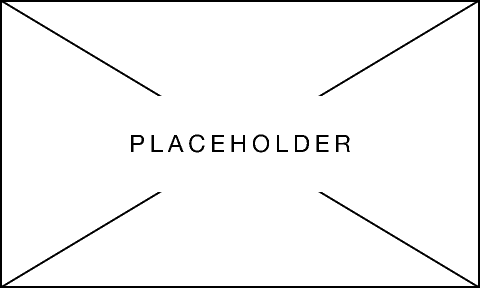
\includegraphics{Images/placeholder.png}
  \centering
  \caption{Image Of the CAD}
  \label{fig:intro:gearbox}
\end{figure}

\paragraph{}
\TODO {Brief description of the strategic advantages in relation to this year's game and how it could be relevant in the future} 
\vspace {1em} \\
\TODO {Positives + Negatives table}

\begin{table}[h]
  \centering
  \begin{tabular}{l|l}
    Positives & Negatives \\ \hline \hline
    1 & 2 \\ \hline
    3 & 4 \\ \hline                          
  \end{tabular}
  \caption{Considerations}
\end{table}

\TODO {Required Tools}
\begin{itemize}
  \item Hand Drill
  \item Jigsaw
\end{itemize}

\newpage

\section{Instructions} \label{sec:Instructions}
\paragraph{ TBW }

\end{document}